%!TEX root=../GaugeCNNTheory.tex


\newpage


\begin{figure}
	\centering
	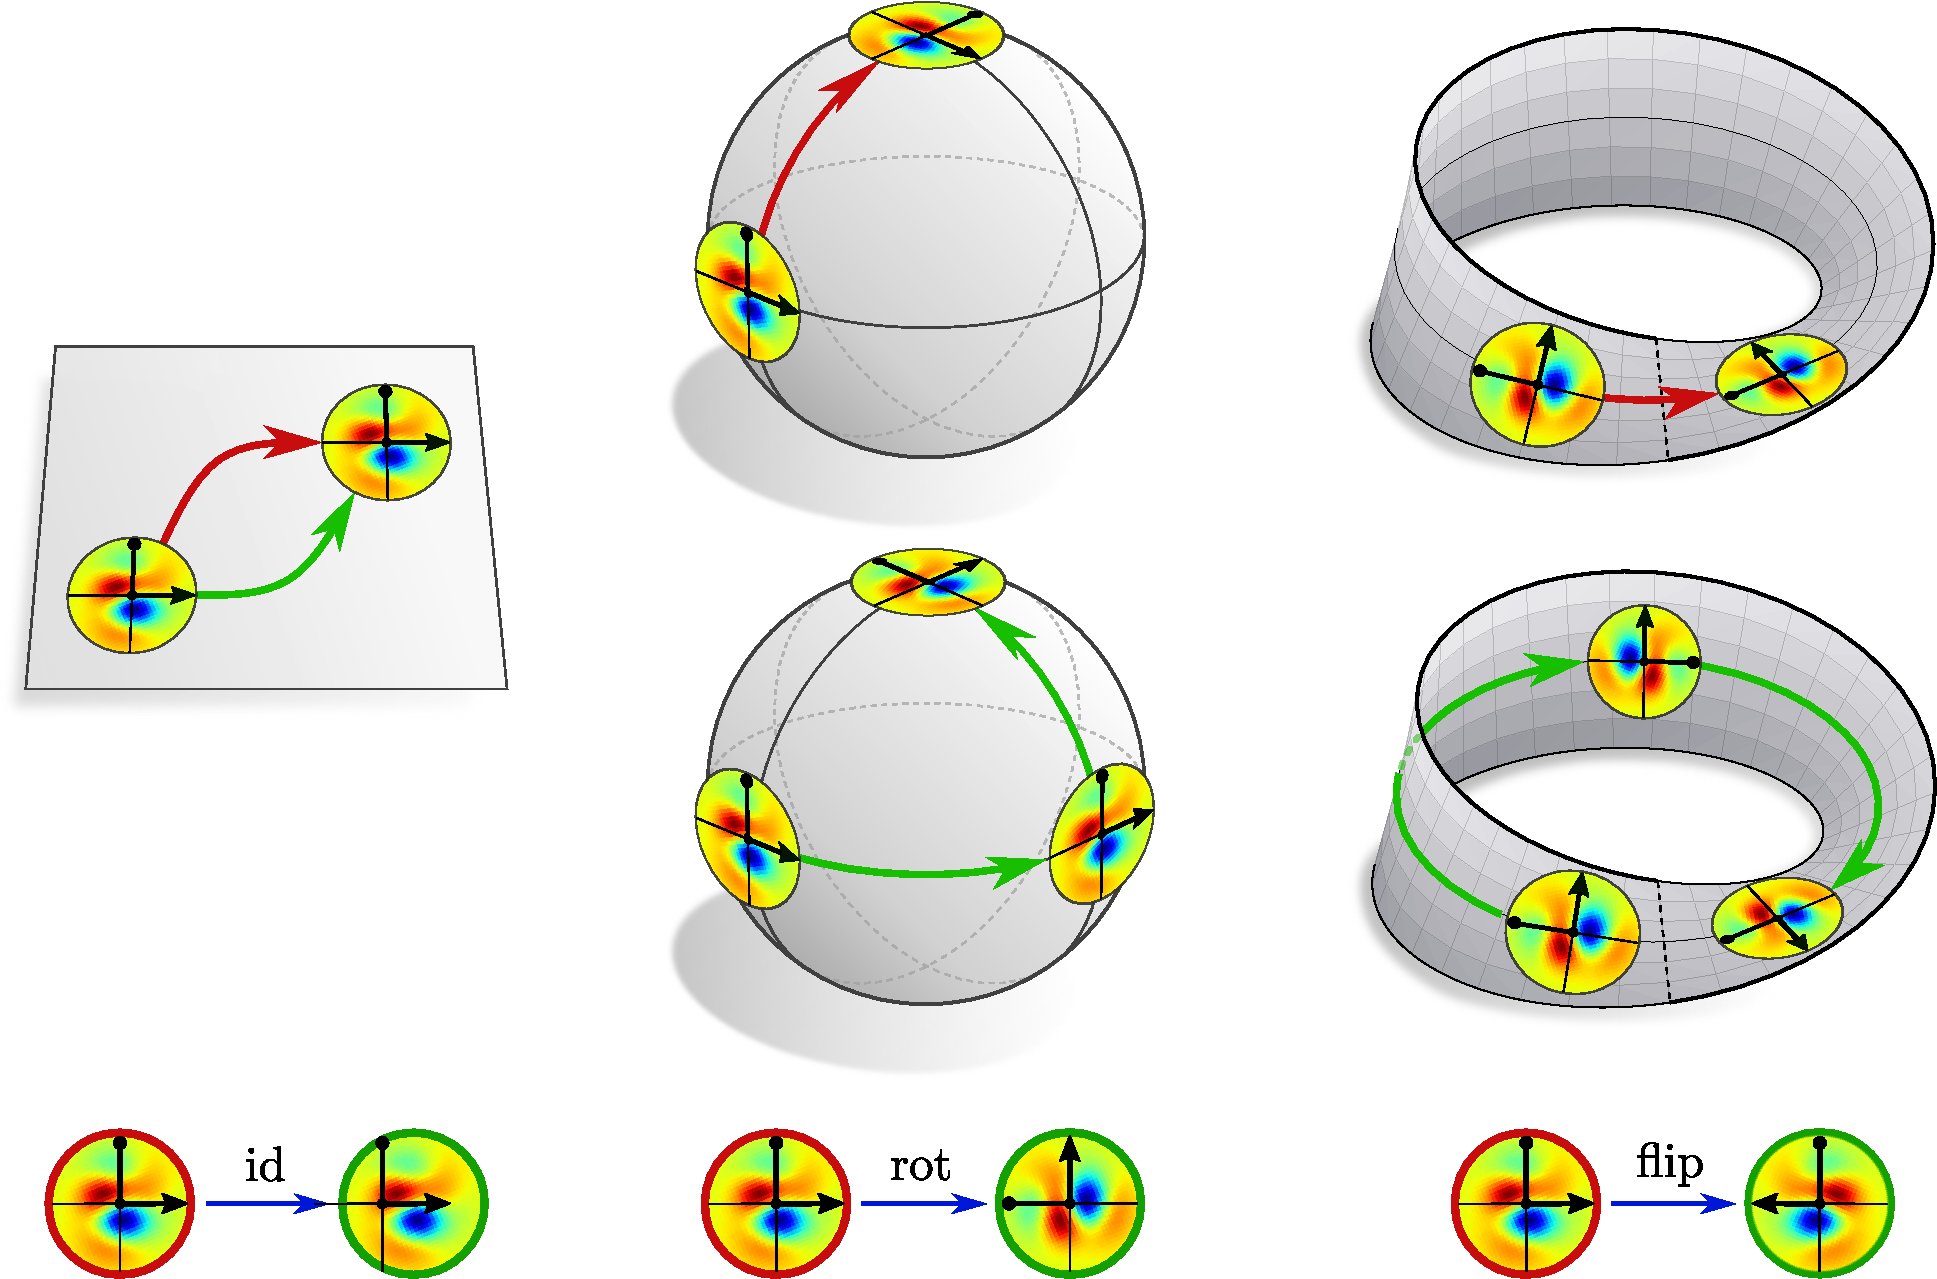
\includegraphics[width=.93\columnwidth]{figures/intro_transport_ambiguity.pdf}
	\caption{\small
		شهودی در مورد ابهام ذاتی اشتراک وزن در منیفلدهایی.
		\ \ \emph{چپ:}
		یک تفسیر رایج از اشتراک وزن در صفحه، جابجایی یک کرنل در کل فضا است.
		از آنجا که انتقال موازی در فضاهای مسطح مستقل از مسیر است، این امر بدون ابهام است.
		\ \ \emph{وسط:}
		در فضاهای خمیده، مانند کره، انتقال موازی وابسته به مسیر است.
		مسیرهای مختلف منجر به کرنل‌هایی می‌شوند که نسبت به یکدیگر چرخانده شده‌اند.
		\ \ \emph{راست:}
		نوار موبیوس یک منیفولد غیرقابل جهت‌گیری است.
		بنابراین، مسیرهای مختلف می‌توانند منجر به کرنل‌هایی شوند که نسبت به یکدیگر بازتاب یافته‌اند.
		\ \ \emph{پایین:}
		ما ترازهای مختلف کرنل را با انتخاب‌های مختلف چارچوب‌های مرجع محلی از فضاهای مماس مربوطه رسمی‌سازی می‌کنیم.
		به خوبی شناخته شده است که هیچ انتخابی از چارچوب‌های مرجع (گیج) در منیفلدهای عمومی ارجح نیست.
		مختصات‌بندی‌های مختلف با تبدیل‌های گیج مرتبط هستند، که مقادیری در گروه ساختار $G$ منیفولد (گروه بدیهی $G=\{e\}$ برای صفحه، گروه چرخش $G=\SO{2}$ برای کره و گروه بازتاب $G = \Flip$ برای نوار موبیوس) می‌گیرند.
		شبکه‌های کانولوشنی مستقل از مختصات، ابهام چارچوب‌های مرجع را با اعمال کرنل‌های کانولوشنی $G$-استیریبل (تناوب‌پذیر گیج) برطرف می‌کنند.
	}
	\label{fig:weight_sharing_ambiguity}
\end{figure}


\section{مرور کلی و شهود بصری}
\label{sec:visual_intro}


فرمول‌بندی جبری شبکه‌های کانولوشنی مستقل از مختصات نیازمند آشنایی با نظریه گروه‌ها، نظریه نمایش‌ها و هندسه دیفرانسیل است که ممکن است برای مخاطبان غیرتخصصی مانعی ایجاد کند.
با این حال، بیشتر ساختارها و نتایج ما از نظر هندسی بسیار شهودی هستند و می‌توان آن‌ها را با چند مثال بصری توضیح داد.
این بخش تلاش می‌کند تا مروری کلی و شهود بصری در مورد شبکه‌های کانولوشنی مستقل از مختصات ارائه دهد.

بخش~\ref{sec:intro_overview_GM_conv} زیر، کانولوشن‌های مستقل از مختصات $\GM$ را در منیفلدهای ریمانی معرفی می‌کند.
تناوب‌پذیری آن‌ها تحت عمل ایزومتری‌ها در بخش~\ref{sec:intro_overview_isometry} مورد بحث قرار می‌گیرد.
بخش~\ref{sec:intro_overview_G_structure_choice} در مورد عواملی که بر انتخاب $G$-ساختار در طراحی شبکه‌های کانولوشنی مستقل از مختصات تأثیر می‌گذارند، توضیح می‌دهد.


\toclesslab\subsection{\textit{G}-ساختارها و کانولوشن‌های مستقل از مختصات \textit{GM}}{sec:intro_overview_GM_conv}
از آنجا که کانولوشن‌ها اساساً با خاصیت اشتراک وزن خود مشخص می‌شوند، یک سؤال اصلی در این کار این است:
\vspace*{-1ex}
\begin{center}\it
	چگونه باید کرنل‌های کانولوشن بر روی منیفلدهای ریمانی به اشتراک گذاشته شوند؟
	\footnote{
		این سؤال به طور کلی‌تر برای هر تابع قالب محلی، به عنوان مثال بایاس‌ها یا غیرخطی‌های نقطه‌ای نیز کاربرد دارد.
	}
\end{center}

%%%%%%%%%%%%%%%%%%%%%%%%%%%%%%%%%%%%%%%%%%%%%%%%%%%%%%%%%%%%%%%%%%%%%%%
%%%%%%%%%%%%%%%%%%%%%%%%%%%%%%%%%%%%%%%%%%%%%%%%%%%%%%%%%%%%%%%%%%%%%%%
\marginnote{} % somehow forces stuff on first page...
%%%%%%%%%%%%%%%%%%%%%%%%%%%%%%%%%%%%%%%%%%%%%%%%%%%%%%%%%%%%%%%%%%%%%%%
%%%%%%%%%%%%%%%%%%%%%%%%%%%%%%%%%%%%%%%%%%%%%%%%%%%%%%%%%%%%%%%%%%%%%%%


یک رویکرد رایج \marginnote{اشتراک وزن از طریق تقارن‌ها} به اشتراک گذاشتن وزن‌ها از طریق عمل یک گروه تقارنی از فضای زیرین است~\cite{Cohen2016-GCNN,Kondor2018-GENERAL}.
به عنوان مثال، شبکه‌های کانولوشنی سنتی وزن‌ها را با جابجایی کرنل‌ها روی صفحه به اشتراک می‌گذارند، در حالی که شبکه‌های کانولوشنی کروی وزن‌ها را با چرخش کرنل‌ها روی کره به اشتراک می‌گذارند.
برای به اشتراک گذاشتن یک کرنل در کل فضا، عمل گروه تقارنی باید \emph{متعدی} باشد.
از آنجا که این امر به طور کلی برای ایزومتری‌های منیفلدهای ریمانی صادق نیست، این استراتژی برای هدف ما رد می‌شود.


اشتراک وزن در فضاهای اقلیدسی اغلب به عنوان "جابجایی" یک کرنل در فضا در نظر گرفته می‌شود.
\marginnote{اشتراک وزن از طریق انتقال}
از آنجا که در فضاهای مسطح انتقال موازی مستقل از مسیر انتخاب شده است، این امر منجر به تراز بدون ابهام کرنل‌ها می‌شود؛ به شکل~\ref{fig:weight_sharing_ambiguity} (چپ) مراجعه کنید.
با این حال، در فضاهای خمیده یا غیرقابل جهت‌گیری، انتقال موازی \emph{وابسته به مسیر} می‌شود و بنابراین برای اشتراک وزن نامناسب است.
شکل~\ref{fig:weight_sharing_ambiguity} (وسط و راست) این مشکل را برای کره و نوار موبیوس مثال می‌زند، جایی که مسیرهای مختلف منجر به تراز متفاوتی از کرنل می‌شوند.


از آنجا که مفهوم "ترازهای کرنل" تا حدی مبهم است
\marginnote{اشتراک وزن در امتداد چارچوب‌ها}
ابتدا باید آن را از نظر ریاضی دقیق کنیم:

\begin{minipage}{\textwidth}
	\begin{center}\it
		ما انتخاب تراز کرنل در نقطه‌ای $p\in M$ \\
		را به عنوان انتخاب یک چارچوب مرجع محلی (گیج)
		از فضای مماس مربوطه $\TpM$ رسمی‌سازی می‌کنیم.
	\end{center}
\end{minipage}

یک چارچوب مرجع در $p\in M$ یک تاپل مرتب $[e_1,\, \dots,\, e_d]$ از $d := \dim(M)$ بردار مماس خطی مستقل $e_i \in \TpM$ است که به عنوان محورهای چارچوب نامیده می‌شوند.
از آنجا که چارچوب‌های مختلف در~$p$ با تبدیل‌های خطی مرتبط هستند، انتخاب‌های مختلف چارچوب‌ها با تغییر شکل‌های کرنل خطی مطابقت دارند.
شکل~\ref{fig:intro_kernel_alignment_trivial} دو انتخاب مختلف از میدان‌های چارچوب را در~$M = \R^2$ نشان می‌دهد.
به اشتراک گذاشتن یک کرنل کانولوشنی در امتداد این میدان‌های چارچوب منجر به \emph{میدان‌های کرنل} (کانولوشنی) مربوطه می‌شود.


شناسایی ترازهای کرنل با چارچوب‌های مرجع این سؤال را مطرح می‌کند:
\begin{center}\it
	انتخاب چارچوب‌های مرجع محلی بر روی یک منیفولد (ریمانی) تا چه حد مبهم است؟
\end{center}
همانطور که در ادامه توضیح داده می‌شود، ابهام چارچوب‌های مرجع توسط یک $G$-ساختار که منیفولد به آن مجهز است، تعیین می‌شود.


\begin{SCfigure}
	\centering
	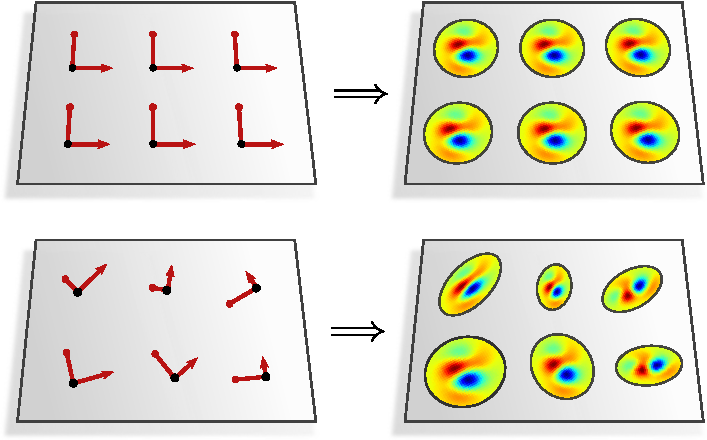
\includegraphics[width=.62\textwidth]{figures/intro_kernel_alignment_trivial.pdf}
	\captionsetup{width=.9\textwidth}
	\caption{\small
		یک ویژگی کلیدی کانولوشن‌ها این است که آن‌ها \emph{وزن‌ها را} در سراسر منیفولد \emph{به اشتراک می‌گذارند}.
		ما تراز یک کرنل در $p\in M$ را با \emph{انتخاب یک چارچوب مرجع} – یا \emph{گیج} – از فضای مماس مربوطه~$\TpM$ شناسایی می‌کنیم.
		بنابراین \emph{میدان‌های چارچوب} مختلف دلالت بر \emph{میدان‌های کرنل} (کانولوشنی) متفاوتی دارند.
		\\[1ex]
		انتخاب چارچوب‌ها اغلب منحصر به فرد نیست.
		ابهام در این انتخاب با $G$-\emph{ساختارها} رسمی‌سازی می‌شود؛ به شکل~\ref{fig:G_structures_intro} مراجعه کنید.
		برای در نظر گرفتن اختیاری بودن چارچوب‌ها، کرنل‌ها ملزم می‌شوند که $G$-استیریبل (تناوب‌پذیر) باشند، همانطور که در اشکال~\ref{fig:intro_steerable_kernel} و~\ref{fig:intro_kernel_alignment_reflect} بصری‌سازی شده است.
		\\[0pt]
	}
	\label{fig:intro_kernel_alignment_trivial}
\end{SCfigure}


\subsubsection{\textit{G}-ساختارها}
\label{sec:visual_intro_GM_subsub}

فضای \emph{همه} چارچوب‌های ممکن $\TpM$ با عنوان~$\FpM$ نشان داده می‌شود.
\marginnote{بندل چارچوب $\FM$}
با هم، چارچوب‌های همه فضاهای مماس، \emph{بندل چارچوب}~$\FM$ را تشکیل می‌دهند؛ به شکل~\ref{fig:frame_bundle} مراجعه کنید.
هیچ انتخاب خاصی از چارچوب‌ها در $\FM$ بر روی یک منیفولد هموار "عریان" (بدون ساختار هندسی اضافی) ترجیح داده نمی‌شود، که ابهام تراز کرنل‌ها را حداکثری می‌کند.
برای رفع ابهام چارچوب‌ها و ترازهای کرنل، منیفولد باید با \emph{ساختار هندسی اضافی} مجهز شود.


یک منیفولد ریمانی با \emph{ساختار متریک} مجهز شده است.
\marginnote{ساختار متریک $\OM$}
با ارائه یک حاصل‌ضرب داخلی (متریک ریمانی) بر روی فضاهای مماس، این ساختار امکان شناسایی چارچوب‌های خاصی را می‌دهد که محورهای آن‌ها \emph{متعامد} با یکدیگر هستند.
\emph{تبدیل‌های گیج}، یعنی تبدیل‌ها بین انتخاب‌های چارچوب‌های مرجع (به اشکال~\ref{fig:intro_gauge_isom_induction} (چپ) و~\ref{fig:gauge_trafos} مراجعه کنید)، سپس مقادیری در \emph{گروه متعامد}~$\O{d}$ می‌گیرند.
در منیفلدهای ریمانی، تراز کرنل‌ها همیشه تا چرخش‌ها و بازتاب‌ها بدون ابهام است.


شبکه‌های کانولوشنی اقلیدسی کرنل‌های کانولوشن (و در نتیجه چارچوب‌ها) را تراز می‌کنند
\marginnote{$G$-ساختارها $\GM$}
موازی با یکدیگر همانطور که در شکل~\ref{fig:intro_kernel_alignment_trivial} (بالا) بصری‌سازی شده است.
شبکه‌های کانولوشنی کروی معمولاً ترازهای کرنل را تا چرخش‌ها بدون ابهام می‌کنند، یعنی آن‌ها یک دست‌پری ترجیحی از چارچوب‌های مرجع را فرض می‌کنند.
ساختار متریک به تنهایی برای توصیف این تنظیمات کافی نیست، که نشان می‌دهد این منیفلدهایی با \emph{ساختار هندسی اضافی علاوه بر ساختار متریک} مجهز شده‌اند.
ما پیشنهاد می‌کنیم که چارچوب ریاضی مناسب، $G$-\emph{ساختارها} است و فرض می‌کنیم:

\begin{minipage}{\textwidth}
	\begin{center}\it
		ابهام در انتخاب چارچوب‌های مرجع (و در نتیجه ترازهای کرنل) \\
		بر روی یک منیفولد $M$ با $G$-ساختار $\GM$ آن رسمی‌سازی می‌شود.
	\end{center}
\end{minipage}

$G$-ساختارها $\GM$ \emph{بندل‌هایی از چارچوب‌های مرجع متمایز} بر روی $M$ هستند به طوری که \emph{تبدیل‌های گیج} بین چارچوب‌های یک فضای مماس واحد، مقادیری در \emph{گروه ساختار}~${G\leq\GL{d}}$ می‌گیرند.
به طور شهودی، می‌توان مجموعه $\GpM$ چارچوب‌های $\TpM$ را "شبیه" $G$ دانست، با این حال، بدون یک مبدأ متمایز.%
\footnote{
	$\GpM$ یک \emph{فضای همگن اصلی} از~$G$ (یا $G$-torsor) است.
}


بندل چارچوب $\FM$ خود یک $G$-ساختار با~${G=\GL{d}}$ است، در حالی که بندل چارچوب‌های متعامد $\OM$ یک $G$-ساختار (ساختار متریک) با~${G=\O{d}}$ است.
شبکه‌های کانولوشنی اقلیدسی سنتی بر روی میدان چارچوب کانونی در $\R^d$ که در شکل~\ref{fig:G_structure_intro_a} نشان داده شده است، تکیه دارند که یک $G$-ساختار برای گروه بدیهی~${G=\{e\}}$ است.
شکل~\ref{fig:G_structures_intro} $G$-ساختارها را برای منیفلدهای بیشتر و گروه‌های ساختار دیگر بصری‌سازی می‌کند.
مروری بر گروه‌های ساختار رایج در جدول~\ref{tab:G_structures} در بخش~\ref{sec:local_G-structure_G-atlas} یافت می‌شود.


ما در ادامه همیشه منیفلدهای ریمانی را مجهز به یک $G$-ساختار اضافی در کنار ساختار متریک خود فرض خواهیم کرد.%
\footnote{
	$G$-ساختار باید با ساختار متریک سازگار باشد به این صورت که چارچوب‌های متمایز در $\GM$ زیرمجموعه‌ای از چارچوب‌های متعامد در $\OM$ باشند زمانی که $G<\O{d}$.
	به طور خاص برای $G=\O{d}$، $G$-ساختار $\GM$ با ساختار متریک $\OM$ منطبق است و اطلاعات هندسی اضافی را اضافه نمی‌کند.
}
انتخاب خاص $G$-ساختار خواص شبکه عصبی را تعیین می‌کند؛ ما در مورد این انتخاب در بخش~\ref{sec:intro_overview_G_structure_choice} زیر توضیح خواهیم داد.


%%%%%%%%%%%%%%%%%%%%%%%%%%%%%%%%%%%%%%%%%%%%%%%%%%%%%%%%%%%%%%%%%%%%%%%%%%%%%%%%%%%%%%%%%%%%%%%%%%%%%%%%%%
\afterpage{ % execute argument of this command *after* end of current page
	\clearpage % clear any pending floats
	%%%%%%%%%%%%%%%%%%%%%%%%%%%%%%%%%%%%%%%%%%%%%%%%%%%%%%%%%%%%%%%%%%%%%%%%%%%%%%%%%%%%%%%%%%%%%%%%%%%%%%%%%%
	\begin{figure}
		\centering
		\vspace*{-4.ex}
		\begin{subfigure}[b]{0.26\textwidth}
	\centering
	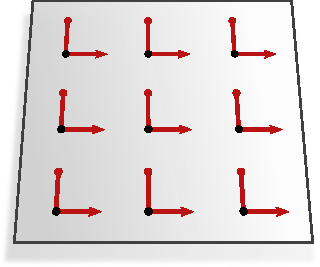
\includegraphics[width=1.\textwidth]{figures/G_structure_R2_1_big.pdf}
	\captionsetup{format=hang}
	\caption{\small
		\,$M = \R^2$,
		\,$G = \{e\}$
	}
	\label{fig:G_structure_intro_a}
\end{subfigure}
\hfill
\begin{subfigure}[b]{0.26\textwidth}
	\centering
	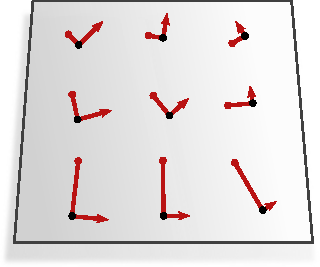
\includegraphics[width=1.\textwidth]{figures/G_structure_R2_5_big.pdf}
	\captionsetup{format=hang}
	\caption{\small
		\,$M = \R^2$,
		\,$G = \{e\}$
	}
	\label{fig:G_structure_intro_b}
\end{subfigure}
\hfill
\begin{subfigure}[b]{0.26\textwidth}
	\centering
	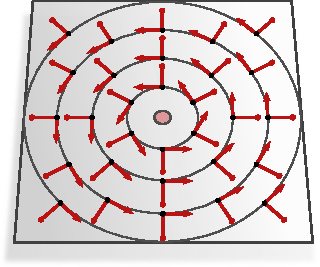
\includegraphics[width=1.\textwidth]{figures/G_structure_R2_no_origin_SO2_intro.pdf}
	\captionsetup{format=hang}
	\caption{\small
		\,$M = \R^2\backslash\{0\}$,
		\,$G = \{e\}$
	}
	\label{fig:G_structure_intro_c}
\end{subfigure}
\\[2ex]
%
%
%
%
\begin{subfigure}[b]{0.26\textwidth}
	\centering
	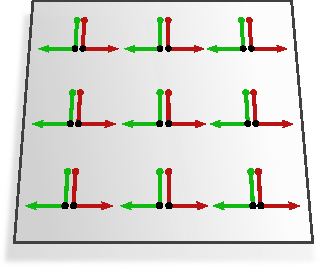
\includegraphics[width=1.\textwidth]{figures/G_structure_R2_3_big.pdf}
	\captionsetup{format=hang}
	\caption{\small
		\,$M = \R^2$,
		\,$G = \Flip$
	}
	\label{fig:G_structure_intro_d}
\end{subfigure}
\hfill
\begin{subfigure}[b]{0.26\textwidth}
	\centering
	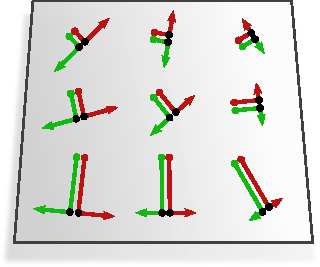
\includegraphics[width=1.\textwidth]{figures/G_structure_R2_6_big.pdf}
	\captionsetup{format=hang}
	\caption{\small
		\,$M = \R^2$,
		\,$G = \Flip$
	}
	\label{fig:G_structure_intro_e}
\end{subfigure}
\hfill
\begin{subfigure}[b]{0.26\textwidth}
	\centering
	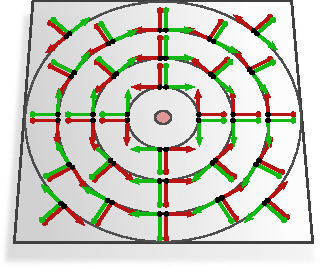
\includegraphics[width=1.\textwidth]{figures/G_structure_R2_no_origin_O2_intro.pdf}
	\captionsetup{format=hang}
	\caption{\small
		\,$M = \R^2\backslash\{0\}$,
		\,$G = \Flip$
	}
	\label{fig:G_structure_intro_f}
\end{subfigure}
\\[2ex]
%
%
%
%
\begin{subfigure}[b]{0.26\textwidth}
	\centering
	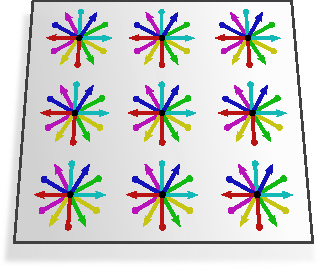
\includegraphics[width=1.\textwidth]{figures/G_structure_R2_2_big.pdf}
	\captionsetup{format=hang}
	\caption{\small
		\,$M = \R^2$,
		\,$G = \SO2$
	}
	\label{fig:G_structure_intro_g}
\end{subfigure}
\hfill
\begin{subfigure}[b]{0.26\textwidth}
	\centering
	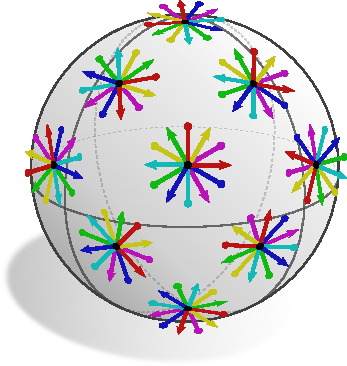
\includegraphics[width=.95\textwidth]{figures/G_structure_S2_1.pdf}
	\vspace*{-2ex}
	\captionsetup{format=hang}
	\caption{\small
		\,$M = S^2$,
		\,$G = \SO2$
	}
	\label{fig:G_structure_intro_h}
\end{subfigure}
\hfill
\begin{subfigure}[b]{0.26\textwidth}
	\centering
	\makebox[\textwidth][c]{ % center over-wide figure
		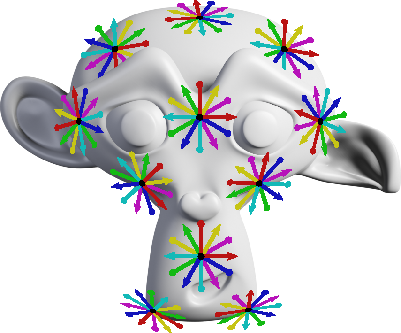
\includegraphics[width=1.12\textwidth]{figures/suzanne_SO2_structure.pdf}
	}
	\vspace*{-3.ex}
	\captionsetup{format=hang, width=1.1\textwidth}
	\caption{\small
		$M = \textup{``\href{https://en.wikipedia.org/wiki/Blender_(software)\#Suzanne}{\lr{Suzanne}}''}$\!,
		\ $G = \SO2$
	}
	\label{fig:G_structure_intro_i}
\end{subfigure}
\\[2ex]
%
%
%
%
\begin{subfigure}[b]{0.26\textwidth}
	\centering
	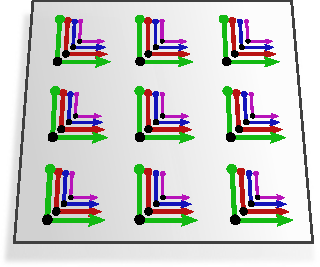
\includegraphics[width=1.\textwidth]{figures/G_structure_R2_4_big.pdf}
	\captionsetup{format=hang}
	\caption{\small
		\,$M = \R^2$,
		\,$G = \Scale$
	}
	\label{fig:G_structure_intro_j}
\end{subfigure}
\hfill
\begin{subfigure}[b]{0.26\textwidth}
	\centering
	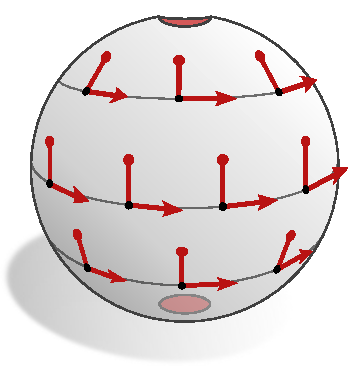
\includegraphics[width=.95\textwidth]{figures/G_structure_S2_2.pdf}
	\vspace*{-2ex}
	\captionsetup{format=hang}
	\caption{\small
		\,$M = S^2\backslash\text{\lr{poles}}$,
		\,$G = \{e\}$
	}
	\label{fig:G_structure_intro_k}
\end{subfigure}
\hfill
\begin{subfigure}[b]{0.26\textwidth}
	\centering
	\makebox[\textwidth][c]{ % center over-wide figure
		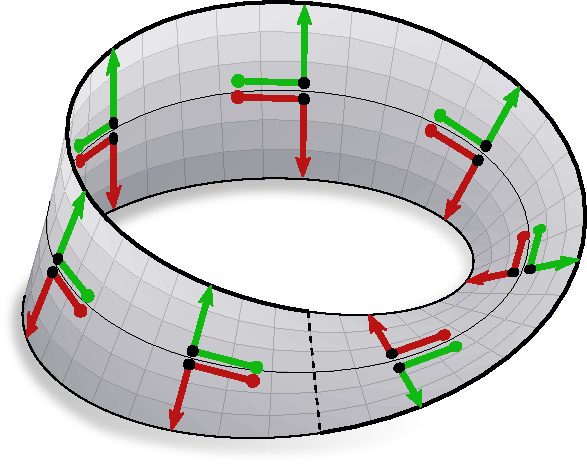
\includegraphics[width=1.1\textwidth]{figures/Mobius_R_structure.pdf}
	}
	\vspace*{-3.ex}
	\captionsetup{format=hang}
	\caption{\small
		\,$M = \textup{\lr{M\"obius}}$,
		\,$G = \Flip$
	}
	\label{fig:G_structure_intro_l}
\end{subfigure} % Assuming this file draws the G-structures.
		\vspace*{1.5ex}
		\captionsetup{width=1.1\textwidth}
		\caption{\small
			نمونه‌ای از $G$-ساختارها $\GM$ برای گروه‌های ساختار $G$ و منیفلدهای $M$ مختلف.
			گروه ساختار $G$ نشان می‌دهد که تبدیل‌های گیج چه مقادیری می‌توانند بگیرند، و بنابراین زیرمجموعه چارچوب‌های متمایز در هر نقطه~$p$ چقدر "بزرگ" است.
			شکل~\ref{fig:G_structure_intro_a} $\{e\}$-ساختار کانونی (میدان چارچوب) در~$\R^2$ را نشان می‌دهد که مربوط به شبکه‌های کانولوشنی اقلیدسی سنتی است.
			\mbox{$G$-ساختارها} در
			اشکال~\ref{fig:G_structure_intro_d}، \ref{fig:G_structure_intro_g} و~\ref{fig:G_structure_intro_j}
			به ترتیب با اضافه کردن چارچوب‌های بازتاب یافته ($G=\Flip$)، چرخانده شده ($G=\SO{2}$) و مقیاس شده ($G=\Scale$) ساخته می‌شوند.
			\GM-کانولوشن‌های مربوطه نه تنها نسبت به انتقال تناوب‌پذیر هستند بلکه تحت عمل گروه‌های آفین~$\Aff(G)$ نیز تناوب‌پذیر می‌باشند.
			\mbox{$G$-ساختارها} معمولاً منحصر به فرد نیستند.
			اشکال~\ref{fig:G_structure_intro_b} و~\ref{fig:G_structure_intro_e} \mbox{$G$-ساختارهای} جایگزین را در~$\R^2$ نشان می‌دهند (مربوط به یک متریک جایگزین که چارچوب‌های آن‌ها نسبت به آن متعامد هستند).
			آن‌ها ممکن است از نظر عملی مرتبط نباشند اما انعطاف‌پذیری چارچوب ما را نشان می‌دهند.
			$\{e\}$-ساختار در شکل~\ref{fig:G_structure_intro_c} مربوط به مختصات قطبی است.
			از آنجا که $G$-ساختارها باید پیوسته باشند، ما مبدأ~$0$ را که مختصات قطبی در آن تکین هستند، حذف کردیم.
			می‌توان بار دیگر یک $\Flip$-ساختار را با اضافه کردن چارچوب‌های بازتاب یافته همانطور که در شکل~\ref{fig:G_structure_intro_f} نشان داده شده است، تعریف کرد.
			این $G$-ساختارها کانولوشن‌ها را در $\R^2\backslash\{0\}$ مدل می‌کنند که نسبت به $\SO{2}$ و $\O{2}$ تناوب‌پذیر هستند اما نسبت به انتقال تناوب‌پذیر نیستند.
			شکل~\ref{fig:G_structure_intro_h} $\SO{2}$-ساختار معمول را در 2-کره (جاسازی شده)~$S^2$ نشان می‌دهد، که زیربنای شبکه‌های کانولوشنی کروی تناوب‌پذیر $\SO{3}$ است.
			یک انتخاب محبوب دیگر $\{e\}$-ساختار در شکل~\ref{fig:G_structure_intro_k} است که توسط مختصات کروی القا می‌شود.
			توجه داشته باشید که این $\{e\}$-ساختار در قطبین تکین خواهد بود، که بنابراین از آن حذف می‌شوند.
			کاهش‌های پیوسته (یعنی غیرتکین) گروه ساختار فراتر از~$\SO{2}$ در کره از نظر توپولوژیکی مسدود شده‌اند.
			بنابراین کرنل‌های $G$-استیریبل با $G\geq\SO{2}$ برای کانولوشن‌های پیوسته در کره‌های توپولوژیکی مانند مش در شکل~\ref{fig:G_structure_intro_i} کاملاً ضروری هستند.
			شکل~\ref{fig:G_structure_intro_l} یک $\Flip$-ساختار را در نوار موبیوس نشان می‌دهد.
			از آنجا که نوار موبیوس غیرقابل جهت‌گیری است، کاهش پیوسته گروه ساختار را فراتر از گروه بازتابی~$G=\Flip$ نمی‌پذیرد.
		}
		\label{fig:G_structures_intro}
		\end{figure>
			%%%%%%%%%%%%%%%%%%%%%%%%%%%%%%%%%%%%%%%%%%%%%%%%%%%%%%%%%%%%%%%%%%%%%%%%%%%%%%%%%%%%%%%%%%%%%%%%%%%%%%%%%%
			\thispagestyle{empty}
			\clearpage % force a page break
		}
		%%%%%%%%%%%%%%%%%%%%%%%%%%%%%%%%%%%%%%%%%%%%%%%%%%%%%%%%%%%%%%%%%%%%%%%%%%%%%%%%%%%%%%%%%%%%%%%%%%%%%%%%%%
		
		
		\subsubsection{\textit{GM}-شبکه‌های مستقل از مختصات}
		هدف ما
		\marginnote{استقلال از مختصات $\GM$ (کوواریانس)}
		طراحی شبکه‌های عصبی بر روی منیفلدهای ریمانی با یک $G$-ساختار اضافی است.
		اگر گروه ساختار $G$ بدیهی نباشد، \emph{هیچ انتخاب کانونی از چارچوب‌های مرجع (گیج) وجود ندارد}.
		با این حال، برای انجام محاسبات عددی، \emph{برخی} گیج، که کرنل‌ها و ویژگی‌ها نسبت به آن بیان می‌شوند، باید انتخاب شود.
		از آنجا که این انتخاب ذاتاً دلخواه است، ما تقاضا می‌کنیم که استنتاج شبکه‌ها در نهایت نباید به آن وابسته باشد، یعنی ما نیاز داریم:
		\begin{center}\it
			شبکه‌های عصبی بر روی یک منیفولد ریمانی با $G$-ساختار $\GM$ \\
			باید بر اساس عملیات "مستقل از مختصات $\GM$" باشند.
		\end{center}
		"استقلال از مختصات $\GM$" در اینجا به این معنی است که \emph{همه کمیت‌های هندسی و توابع بین آن‌ها باید به همان اندازه به خوبی در هر گیج قابل بیان باشند}، یعنی نسبت به هر انتخابی از چارچوب‌های مرجع $G$-ساختار.
		حالت خاص ضرایب بردار مماس و تبدیل‌های گیج بین آن‌ها در شکل~\ref{fig:gauge_trafos} بصری‌سازی شده است.
		شکل~\ref{sec:gauges_TpM_functions} مثالی از یک نگاشت خطی و نمایش مستقل از مختصات آن بر حسب ماتریس‌ها نسبت به چارچوب‌های مختلف را نشان می‌دهد.
		
		
		توجه داشته باشید که نیاز به استقلال از مختصات $\GM$ کاملاً انعطاف‌پذیر است:
		برای $G=\GL{d}$، ما $\GM=\FM$ را داریم و بنابراین حداکثر سطح استقلال از مختصات را.
		در انتهای دیگر طیف گروه‌های ساختار، $G=\{e\}$ قرار دارد، که برای آن $\GM$ یک میدان چارچوب ثابت است و استقلال از مختصات $\GM$ به وابستگی صریح به مختصات کاهش می‌یابد.
		آزادی انتخاب $G$-ساختارهای دلخواه امکان کنترل دقیق بر استقلال از مختصات شبکه‌ها را فراهم می‌کند،
		که در عمل به طور گسترده‌ای متفاوت است؛ به عنوان مثال به جدول~\ref{tab:network_instantiations} در بخش~\ref{part:literature_review} مراجعه کنید.
		
		
		شبکه‌های ما \emph{میدان‌های بردار ویژگی} را بر روی منیفولد پردازش می‌کنند.
		\marginnote{میدان‌های بردار ویژگی مرتبط با $G$}
		بردارهای ویژگی کمیت‌های هندسی \emph{مستقل از مختصات} هستند، مانند بردارهای مماس.
		نسبت به یک چارچوب (گیج) انتخاب شده، آن‌ها را می‌توان با \emph{بردارهای ضریب عددی} نمایش داد.
		نیاز به استقلال از مختصات $\GM$ ایجاب می‌کند که ضرایب عددی در گیج‌های مختلف، محتوای اطلاعاتی یکسانی را کدگذاری کنند.
		این امر به طور طبیعی با مرتبط کردن ویژگی‌ها با یک نمایش گروهی~$\rho$ از گروه ساختار~$G$ حاصل می‌شود که قانون تبدیل ضرایب آن‌ها را تحت تبدیل‌های گیج تعیین می‌کند:
		\begin{center}\it
			میدان‌های بردار ویژگی با یک نمایش $G$ ($\rho$) مرتبط هستند که \\
			قانون تبدیل ضرایب عددی آن‌ها را هنگام تبدیل بین چارچوب‌های مرجع مشخص می‌کند.
			\\[1ex]
			از نظر فنی، میدان‌های ویژگی برش‌هایی از بندل‌های بردار ویژگی مرتبط با $G$ هستند.
			\end{center>
				مثال‌های معمول میدان‌های اسکالر، میدان‌های بردار مماس یا سایر میدان‌های تانسور هستند، با این حال، هر قانون تبدیلی مجاز است و می‌تواند توسط کاربر انتخاب شود.
				انتخاب‌های رایج دیگر برای~$\rho$ در زمینه یادگیری عمیق، نمایش‌های کاهش‌ناپذیر یا منظم هستند؛
				مثال‌های بیشتر در جدول~\ref{tab:network_instantiations} در بخش~\ref{part:literature_review} فهرست شده‌اند.
				
				
				ما می‌خواهیم تأکید کنیم که نیاز به استقلال از مختصات $\GM$ صرفاً یک \emph{شرط سازگاری} است، که تضمین می‌کند مشاهده‌گران مختلف (چارچوب‌ها) بر روی مشاهده هندسی مستقل از مختصات یکسانی توافق دارند.
				این امر مجموعه توابع مجاز را به هیچ وجه محدود \emph{نمی‌کند}، بلکه فقط چگونگی ارتباط عبارات آن‌ها نسبت به چارچوب‌های مختلف را مشخص می‌کند.
				به طور خاص، \emph{شبکه‌های عصبی مستقل از مختصات $\GM$ به طور کلی نیازی به تناوب‌پذیری گیج ندارند}.
				نیاز به تناوب‌پذیری گیج زمانی مطرح می‌شود که اشتراک وزن و استقلال از مختصات به طور همزمان طلب شود، یعنی کانولوشن‌های مستقل از مختصات $\GM$ بر روی کرنل‌های تناوب‌پذیر گیج تکیه دارند.